% Chapter 3
%
\chapter{Concept and Design of SendIt} % Main chapter title
%
	%Concepts
		%First trust
		%Trust building & factors (timing etc)
		%Authentication
			
	%SendIt program
		%Key Management & generation
			%How, why like this, where stored
	
		%Encryption & Decryption
			%Verify identity, how-to?, symkey + key-pairs 
	
		%Connection setup - Offer&Answer generation & Processing
			%webrtc, ice & sdp, what is shared (IV, symkey, cipher)
	
		%Protocol
		
		%File transfer
		
		%Modes
	%ACS Server
		%Authentication

		%WS

		%Protocol
	
	%Program Flow

		%Installation and launch

		%Home screen

		%Settings screen
	
	%extendability?


\label{Chapter3} % For referencing the chapter elsewhere, use \ref{Chapter1} 
%
%TODO Intro!
This chapter will discuss the implementation and use of the solutions discussed in \Cref{Chapter2}. It will illustrate how SendIt utilizes the solutions and how this is beneficial to the system as a whole. In addition, other general information and implementations relevant to the application and system as a whole, will be discussed here.

%
\section{Concepts}
%Concepts
%Todo Review
These concepts and assumptions build the base of how the technology is applied, while also being a product of the technological limitations and how this technology is implemented. The concepts introduced are a mix of new concepts and ideas and concepts borrowed from previous research. The assumptions are a result and consequence of the initial idea of the system, as well as the technological limitations imposed by the chosen technologies, combined with the lack of better options. These were necessary to narrow down the work and to be able to keep the system simple for the end-users. While these may limit or reduce some of the security measures available, the limitations they would impose on the usability is considered more important.

%
	\subsection{First trust}
		%TODO REVIEW
		The first trust or initial trust, is the basis of every interaction in every computer system, as well as in the real world. In the real world, you can see the other person and as such easily identify who it is. This is not the case in computer systems and as such a way to identify entities is necessary. In this system, the choice was made to use e-mail addresses as a basis for uniquely identifying each entity. Since one of the main goals is to improve e-mail attachments, it felt like a natural choice, as well as being easy to implement. Since there is now a way to address each entity, the necessity for confirming that identity arises. This process is called authentication, and how it is done will be discussed more in depth later.

		To able to authenticate an identity, we need to address the fact that that identity has to possess something unique. If not, someone else can impersonate them. In the real world, we each have a unique, or close to unique appearance, which is almost impossible to fake. This is not the case for computers. Usually the PKI model (explained in \Cref{sec:pkc}), is used to vouch for the validity of an identity in computer systems. As explained previously, this requires a lot of setup and cannot be easily done. Because of this, it is not fit to be used in combination with SendIt. 

		SendIt is built on the idea of trusting the first interaction, based on non-absolute authentication methods. This means the first answer and offer exchange (connection setup) is done assuming the other endpoint is not malicious. It is done in an unencrypted manner, without any guarantee of the integrity of the message or using any authentication mechanisms. The reason for choosing this solution is that it allows for an easy and convenient way to start communicating with new partners. It is important that the system is kept simple, to make sure it stays user friendly.

		It also allows for an intuitive approach to the first interaction. Instead of having someone pre-shared secret or other means of verification, the timing and files shared can be a means of verification. It feels unnatural to have someone randomly send files to you unless it is expected. It is also strange to receive files where the content seems unknown or strange, without any previous communication or knowledge. As such, the argument can be made that this system is more intuitive than the alternatives.

		While the timing and files shared do continue to count towards the trust in an identity, it is important to note that \emph{only the first interaction is inherently trusted}. All subsequent communication is end to end encrypted and the endpoint \emph{is always authenticated} before communication starts. As such, if the user takes care to be certain of the endpoints identity for the first interaction, all subsequent interactions are guaranteed to be with the same identity, barring that person having their credentials stolen.

		The take away from this is that, while the timing and files shared should still be considered, all subsequent interactions are by and large guaranteed to be with the same identity. As such users are encouraged to take extra care during the initial setup, but can relax and assume good faith on all future interactions and rely on the system to warn them if something is amiss.

		To sum it up by using a comparative example: If someone were to place a random package outside your door at a random time, with no information on it, one would naturally be wary of the contents and motives of that person. In contrast, if a friend made an appointment to deliver a package that day, one would be much less suspicions, even if it looked identical to the one in the previous scenario. There is no guarantee that the package is from your friend, but it is likely.

		This is the basis of the first trust in SendIt, and allows for an unauthenticated interaction to be the basis of the trust building.  The added benefit is that unlike in the real world, SendIt can guarantee that the package is unaltered and from your friend for \emph{every interaction after the first one}, no matter when it is delivered and what the package may look like.

		There is no denying that this decision leaves the system and end-user open to be attacked during this first interaction. The advantage is that it keeps the system easy to use and allows for a relatively secure system where one rely on human, intuitive factors for establishing the first trust and machine made, absolute authentication from that point on.

	%
	\subsection{Trust building}
		%TODO REVIEW
		Trust-building in the suggested system is based on several factors. Before getting in to the specifics, it is necessary to point out that the trust system is only a theoretical approach and has not been implemented in the prototype. The proposed system uses trust transitivity \cite{lcns_semantic} (\emph{Trusting in Alice and Alice trusting Bob, means that we trust Bob more, than if Alice was not involved}).

		Other means of building trust includes frequency of communication and bi-directional communication (Acting as both sender and receiver with the same identities involved). Trust built by such activities will gradually accumulate, in contrast to transitive trust. Transitive trust is just a way of assigning an identity an initial trust level based on the introducer's of that identity, and their respective level of trust in said identity. (\emph{How many trusted identities signed, how much do we trust those identities and how much do they trust the certificate?})

		Trust can also be reduced. One event that can cause this is if a user tries to communicate with a previous partner, but that partner is not authenticated according to the key associated with that partner. SendIt's trust system works in a way that gives more weight to reduction in trust. This means it will be harder to gain trust, than to lose it. This is because it is generally a safer approach to be wary, than to assume good faith. In other words, a negative incident will reduce the trust significantly more than a positive incident will increase it. This will help maintain a balanced system that detects untrusted behavior rapidly and acts accordingly.

		%\paragraph{}
		Trust is shared by using certificates. Unlike regular certificates (see \Cref{sec:cert}), SendIt proposes a minimal and simple solution. It proposes that a certificate is just a list of identities and the corresponding cipher. The cipher is made by encrypting the public key of the identity being vouched for, with the users own private key. This way all that is needed to verify the authenticity of a key, is to find the introducer's public key and decrypt the cipher. As such, certificates will contain these fields: Introducer's name, Cipher and Trust. The cipher is as described above. The trust field is a value of either 1 or 2, where 1 indicates full trust and 2 indicates partial trust. The trust value is included so we can assess how much trust the introducer has in the introduced key.
		%
		\begin{figure}
		  \centering
		  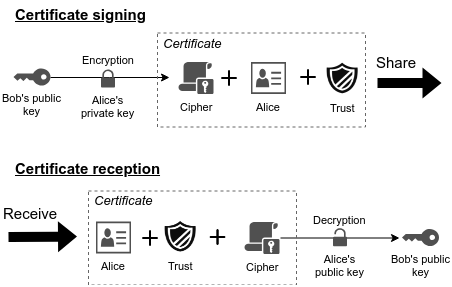
\includegraphics[width=85mm]{Certificate_explained}\\
		  \vspace{1cm}
		  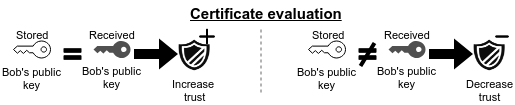
\includegraphics[width=85mm]{Certificate_eval}
		  \centering
		  \decoRule
		  \caption[Certificate operations]{Certificate operations example where Alice signs Bob's certificate.}
		  \label{fig:cert_ex}
		\end{figure}
		%

		When it comes to transitive trust, the specific values and model for assigning trust is not specified, but the idea was to assign different levels of trust based on the amount of introducer's from different trust levels. The level of trust a user has in the introducer of a certificate, directly affects the trust level given to the certificate.

		Once an endpoint has received the certificates, they will be evaluated based on the signatures attached and potentially existing trust values. When the value has been calculated and the new trust level assigned, the key is available like any other and will be used in communications with that identity. See \Cref{fig:cert_ex} for an example. Do note that one certificate can hold many signatures.

		%\paragraph{}
		The practical evaluation scheme for the system is not implemented in SendIt, but the original idea was to assign these trust-levels based on a point system, where an identity accumulates points by getting verified by introducers that the user trusts. An option is to have different levels of trust, where an identity is assigned a trust level according to the amount of points it has accumulated.

		The amount of points granted for each introducer depends on the trust level the user assigns to the introducer. It also depends on how much this introducer trusts in the key. This is so the nuance of transitive trust is clearer, since the system is based on these nuances of trust. SendIt should have an easy and intuitive trust evaluation, while also having a simple way to fairly assert the trust level of an identity. Unlike the web of trust model, different levels of trust for communication and referring should not be applied. There should only be one trust level assigned to each identity and it should apply to both uses equally.

		The practical impact of the different trust levels will be visible to the user as a warning, if the receiver does not have a trust level that is sufficient, according to the users settings. The user should be able to choose if he wants to ignore the warning or cancel the transfer. If the receiver meets the requirements, no notifications or warnings should appear.

		SendIt should come with pre-configured values so novice users can rely on the standard settings. If they want to change these settings, they should have the option to choose to do so. The users will have an overview of all identities and should also have an overview of the respective trust-levels available in the settings-menu, and the option to manually change these levels. This allows the users to override the system in cases where they deem themselves better equipped to evaluate the trust-level of the identity.

		%\paragraph{}
		As noted in \Cref{sec:trust_syl}, the Sylbil attack is a problem in decentralized, reputation based networks. The proposed system will not be completely immune to such attacks, but instead look towards making it hard to propagate and become regarded as trustworthy by the majority of identities. This will be achieved by requiring interactions with other identities, as well as a signed certificate from trusted introducer's, to gain a high level of trust. By requiring these in combination, an attacker can not simply create a large sub-network of controlled identities that all trust each other, and then spread it to the main network with the same level of trust.

		This allows for high resistance against this attack, since the attack exploits the fact that a large number of untrusted identities can manipulate how the main network regards the attacker. Since none of these identities will have a high amount of trust in the main network, they will not be regarded as safe. This is true even if they have a large amount of introducers, because the introducers are untrusted identities as well.

	%
	\subsection{Authentication}
		%Authentication

		The authentication scheme in SendIt is based on the public key cryptography. Each identity, or e-mail address if you will, is associated with a unique public and private key pair. These key pairs are used for authentication. In practice this is done by encrypting the offer and the answer used to establish the WebRTC connection, with the other endpoints public key. This way the ability to connect to each other also acts as authentication, since only the identity with the correct private key can access the information. The above explanation is a slight simplification and will be discussed more in detail, in \Cref{sec:crypto}.

		This is in contrast to usual solutions, where authentication is done before initiating a connection. SendIt's solution removes the extra step, and combines these two processes into one. The reason this is made possible is because of how WebRTC's connection setup is done. Because of the authentication built in to the offer and answer exchange, the system guarantees authentication of both endpoints. For more details on WebRTC's built in authentication of endpoints, see \Cref{sec:conn_setup}.

		As noted above, the authentication in SendIt relies on key pairs. The keys associated with an identity is shared during the first interaction. While there is no authentication of the respective identities during this interaction, the keys are shared over the P2P channel. This channel is end to end encrypted, as to not be vulnerable to attacks that manipulate the data in transit. In summary, as long as you connect to the correct endpoint in your first interaction, there is no reasonable way an attacker can impersonate that endpoint at a later time.

		It is also important to notice that while the proposed system suggests using e-mail addresses as identifiers, there is no direct connection between the identities in the system and the actual e-mail system. By using e-mail addresses, it does make it easier to add extra trust, by implementing an e-mail verification step if desired. The consequence of this initial separation does mean that the e-mail system has no direct influence or inherent effect on SendIt, but their close relation makes it easy to link the two. This gives all the benefit of the e-mail system, while not having to consider the risks or threats that are inherent to that system. It is left up to the developers and users of SendIt to decide if they believe such a link is an positive or negative addition, and as such their choice to make.

%			
\section{SendIt's implementation}
%SendIt implementation
%TODO Review
The following section will address the specific implementation of the general solutions used in SendIt. It will explore the functionality that is used for both modes and explain how they work and why they are necessary. It will also build the basis for understanding how the two modes operate and which functions they build upon to be able to work.

	%
	\subsection{Cryptography}
	\label{sec:crypto}
%
	\begin{figure}[th]
	  \centering
	  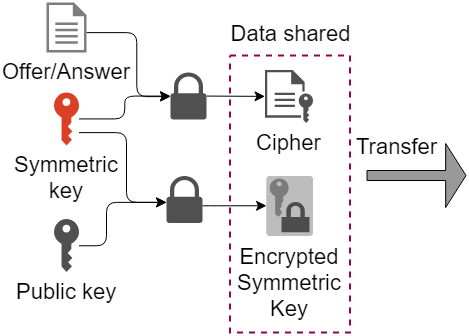
\includegraphics[width=100mm]{Figures/Encrypt}
	  \decoRule
	  \caption[Authentication exchange encryption]{In this figure it is shown how the offer/answer is encrypted with a symmetric key, creating a cipher. This symmetric key is then encrypted with the recipients public key. The cipher and the encrypted key is then shared.}
	  \label{fig:enc}
	\end{figure}
	\begin{figure}[th]
	  \centering
	  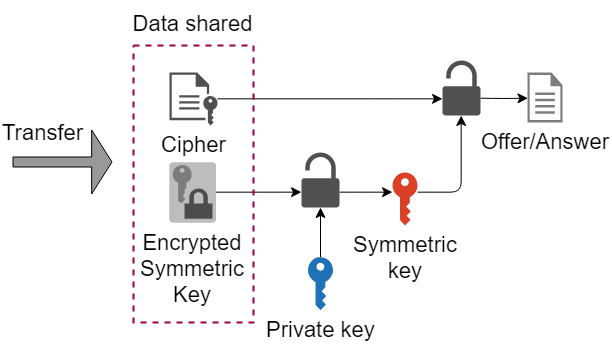
\includegraphics[width=100mm]{Figures/Decrypt}
	  \decoRule
	  \caption[Authentication exchange decryption]{Here one can see the received data and how it is decrypted back into the original offer/answer. Only the identity with the correct private key can access the original data.}
	  \label{fig:decr}
	\end{figure}

	In SendIt's implementation, the Web Crypto API (SubtleCrypto module) is used for generating and handling keys \cite{ar_webcrypto}. This allows for an easy and reliable way to standardize the handling of keys, encryption and decryption in every system. It is available through the Chrome browser, from version 37 \cite{url_webcr_supp}. Using a pre-developed and tested API for SendIts cryptographic functions allows for a more reliable system and more focus on developing new functionality, since the implementation of the cryptographic functions and debugging these is already done. This is the reasoning for using the Web Crypto API.

	The system begins with creating a unique key-pair, if no such key-pair already exists. This check is done at the time of choosing to send or receive a file, so that if desired, the user can change to the correct identity for this connection. The key-pairs used consists of two RSA-OAEP 2048 bit keys with SHA-1 hashing, but this is trivial to change if the need arises. The choice of key-type was based on the recommendation of the WebCrypto API specification \cite{ar_webcrypto}.

	The created key-pair is not stored on disk until the public key has been successfully exchanged with another identity, to avoid storing unnecessary keys. The file where the keys are stored should be password protected or otherwise encrypted, to ensure that if it is stolen, it is not trivial to steal the keys. This is not currently implemented, because of time constraints. 

	The key-exchange is done over the secure data channel created by WebRTCs PeerConnection \cite{ar_webrtc}. Once a key exchange (successful connection) has taken place, the created key-pair and the other identity's public key will be written to disk.

	SendIt imports the file in to memory, once a key is needed. After which it extracts the keys stored. Once the keys have been used and the communication has finished, SendIt will overwrite the existing file with new, updated information. The file containing the keys, stores information exceeding just the known keys. Both the identity associated with a key, and the key itself has to be stored.

	While every identity need to store and keep control over their key pair, SendIt also utilizes symmetric keys for encrypting data. These symmetric keys are generated for every session, and used for one session only. The reason we need to use symmetric keys is because the amount of data that can be encrypted with public key cryptography is fairly small, and as such there is a need for symmetric keys. The maximum amount of data the key pair mentioned above can encrypt is 214 bytes \cite{PKCSV2RSA2012}. SendIt uses an AES-GCM with a length of 256 bits as its symmetric key, which allows for encryption of up to 2\textsuperscript{39} - 256 bytes of data \cite{ar_webcrypto}. This is well within the limits of what is necessary in SendIt. 

	The biggest difference between the symmetric keys and the asymmetric key pairs, is that the symmetric keys are not stored across multiple sessions. The asymmetric keys however, are stored and stay the same. This is because they are used for authenticating the identities. The way this is done, is in a similar fashion to standard PGP encryption and decryption showed in \Cref{sec:pgp_enc}. Look at \Cref{fig:enc} and \Cref{fig:decr} for illustrations on respectively encryption and decryption. The plaintext in this case, is a JavaScript object containing the offer or the answer. If it is encrypted, it also contains the encrypted symmetric key, as well as the initialization vector for that key. The initialization vector consists of 12 random integers. The IV is needed to correctly decrypt the data. 

	The difference between SendIt and PGP is that in order to authenticate the Sender, the recipient needs to encrypt the IV with the Senders public key and transfer this. If a connection is made, it means both endpoints had to have the correct keys. This is because of the way the connection setup of WebRTC works, as described in \Cref{sec:webrtc_off}.
	
	%
	\subsection{Connection setup}
	\label{sec:conn_set_imp}
	%Connection setup - Offer&Answer generation & Processing
			SendIt achieves this by implementing two different ways to create a peer-to-peer connection between two endpoints. These two modes will be explained in \Cref{Chapter4}.

			%Offer / Answer generation
			The offer and answer generation and processing is done as described in \Cref{sec:webrtc}. The difference from the normal usage is that they can also be encrypted before being transferred, which means they have to be decrypted before being used. The original form of the data is a JavaScript object.

			To encrypt the data, it is first turned into a string, then to an ArrayBuffer, after which it is encrypted. To decrypt the data, it is converted from a string to an array of values. Then it is converted to an Uint8Array before being decrypted. The decrypted data is also an Uint8Array, which is turned into a string, and then back to a JavaScript Object. For more information on how the data is exchanged, see \Cref{Chapter4}.

			%ICE and SDP? How and waht differs?
			The actual setup of the connection and the creation of the DataChannel is done according to the examples and descriptions in \Cref{sec:webrtc}. The only difference in connection setup between the two modes, is if ICE-trickling is used or not.

			When the above offer and answer is successfully exchanged, a direct connection is created. There are scenarios, when this is not case though. Known causes of issues with completing the connection are:
			%
			\begin{itemize}
			\item Set-up not completed within a certain time-frame
			\item One or both endpoints are behind symmetrical NAT
			\item One or both endpoints change network location (For example, connect to a different network.)
			\end{itemize}
			%

			When implementing SendIt, the choice was made to not support symmetrical NAT, as it requires a TURN-server. This means the connection would no longer be a direct end-to-end connection. We hope that more people will start using IPv6, as NAT traversal will no longer be necessary. As for changes in network-conditions, there is nothing to be done on the application-side, except including a signaling-server. As such we assume that users will stay in the same network-conditions for the duration the connection is active. For the ACS mode, automatic reconnection is an option which can be added as an extra feature.
	%
	\subsection{Protocol}
	%FT protocol
		%How? Which fields? Additions?
	The base protocol used in SendIt is based on the one used in PubShare, an online, WebRTC P2P file-transfer solution \cite{url_pubshare}. This protocol has been extended and altered to fit with SendIt's needs. This protocol takes care of communicating the status of the file transfer, chunking the data, sharing file meta-data, and verification of complete transfer. The protocol is also in charge of setting up authentication of the endpoints, since the data to authenticate each other should be exchanged directly. This protocol is very limited and as such unlikely to have a large overhead and impact on performance, but this is only an assumption. Following will be a description of the different functionalities of the protocol.

	\subsubsection*{Authentication setup}
	The authentication setup functionality, consist of an Authentication setup package and an Authentication setup reply package. Both of these packages contain the identity and their associated public key. If one of these packages are received, the system checks that the information supplied does not conflict with existing data. If it does not, and the packages was of the type Authentication setup, the endpoint creates an Authentication setup reply package and sends it back. If it was of the type Authentication setup reply, the transfer is initiated.

	\subsubsection*{Offer and Answer}
	The offer packet contains metadata about the files to be sent, so the recipient knows how many files will be transferred, what type of files they are, and how big they are. The Answer packet is just a confirmation that this data was received and that the recipient is getting ready for the transfer.

	\subsubsection*{Request and Data}
	Once the recipient is ready to receive the first data, a Request packet is sent indicating which chunks it wants to receive. It is also used to confirming which packets it has previously received and to request more data, once all the previous chunks has been received. The Data packet contains information about which chunk is being sent, and the filedata for that chunk - the part of the file transferred, in more understandable terms. Following is an example to illustrate how it works:\\
	The recipient sends a Request packet requesting chunks 10 through 20. This also confirms all chunks up until 10 is complete. The Sender then transfers these chunks to the recipient. Once all chunks are received, it requests more chunks, until all chunks have been received. If a chunk is not received, the chunk before is treated as the last chunk received, and the chunks afterwards are re-transmitted.

	\subsubsection*{Done}
	The Done packet contains no data, and is a confirmation that the Recipient has received the current file being transferred. If there are no more files to transfer, this indicates the end of the connection. If more files are waiting, transfer of the next one will begin, once this packet is received.

	\subsubsection*{Cancel and Error}
	The Cancel packet is sent if the user for some reason decides to cancel the current transfer. This interrupts the transfer and closes the connection. If the Error packet is sent, it means an error occurred and the transfer is stopped and the connection closed.

	\subsubsection*{Request metadata}
	The Request metadata packet is only used in the ACS mode. It is needed because in the ACS mode, so the Recipient can request data about which files is being offered by the Sender, before accepting the connection. 

	%
	\subsection{File transfer functionality}
	%File transfer
		%
		\begin{figure}[th]
		  \centering
		  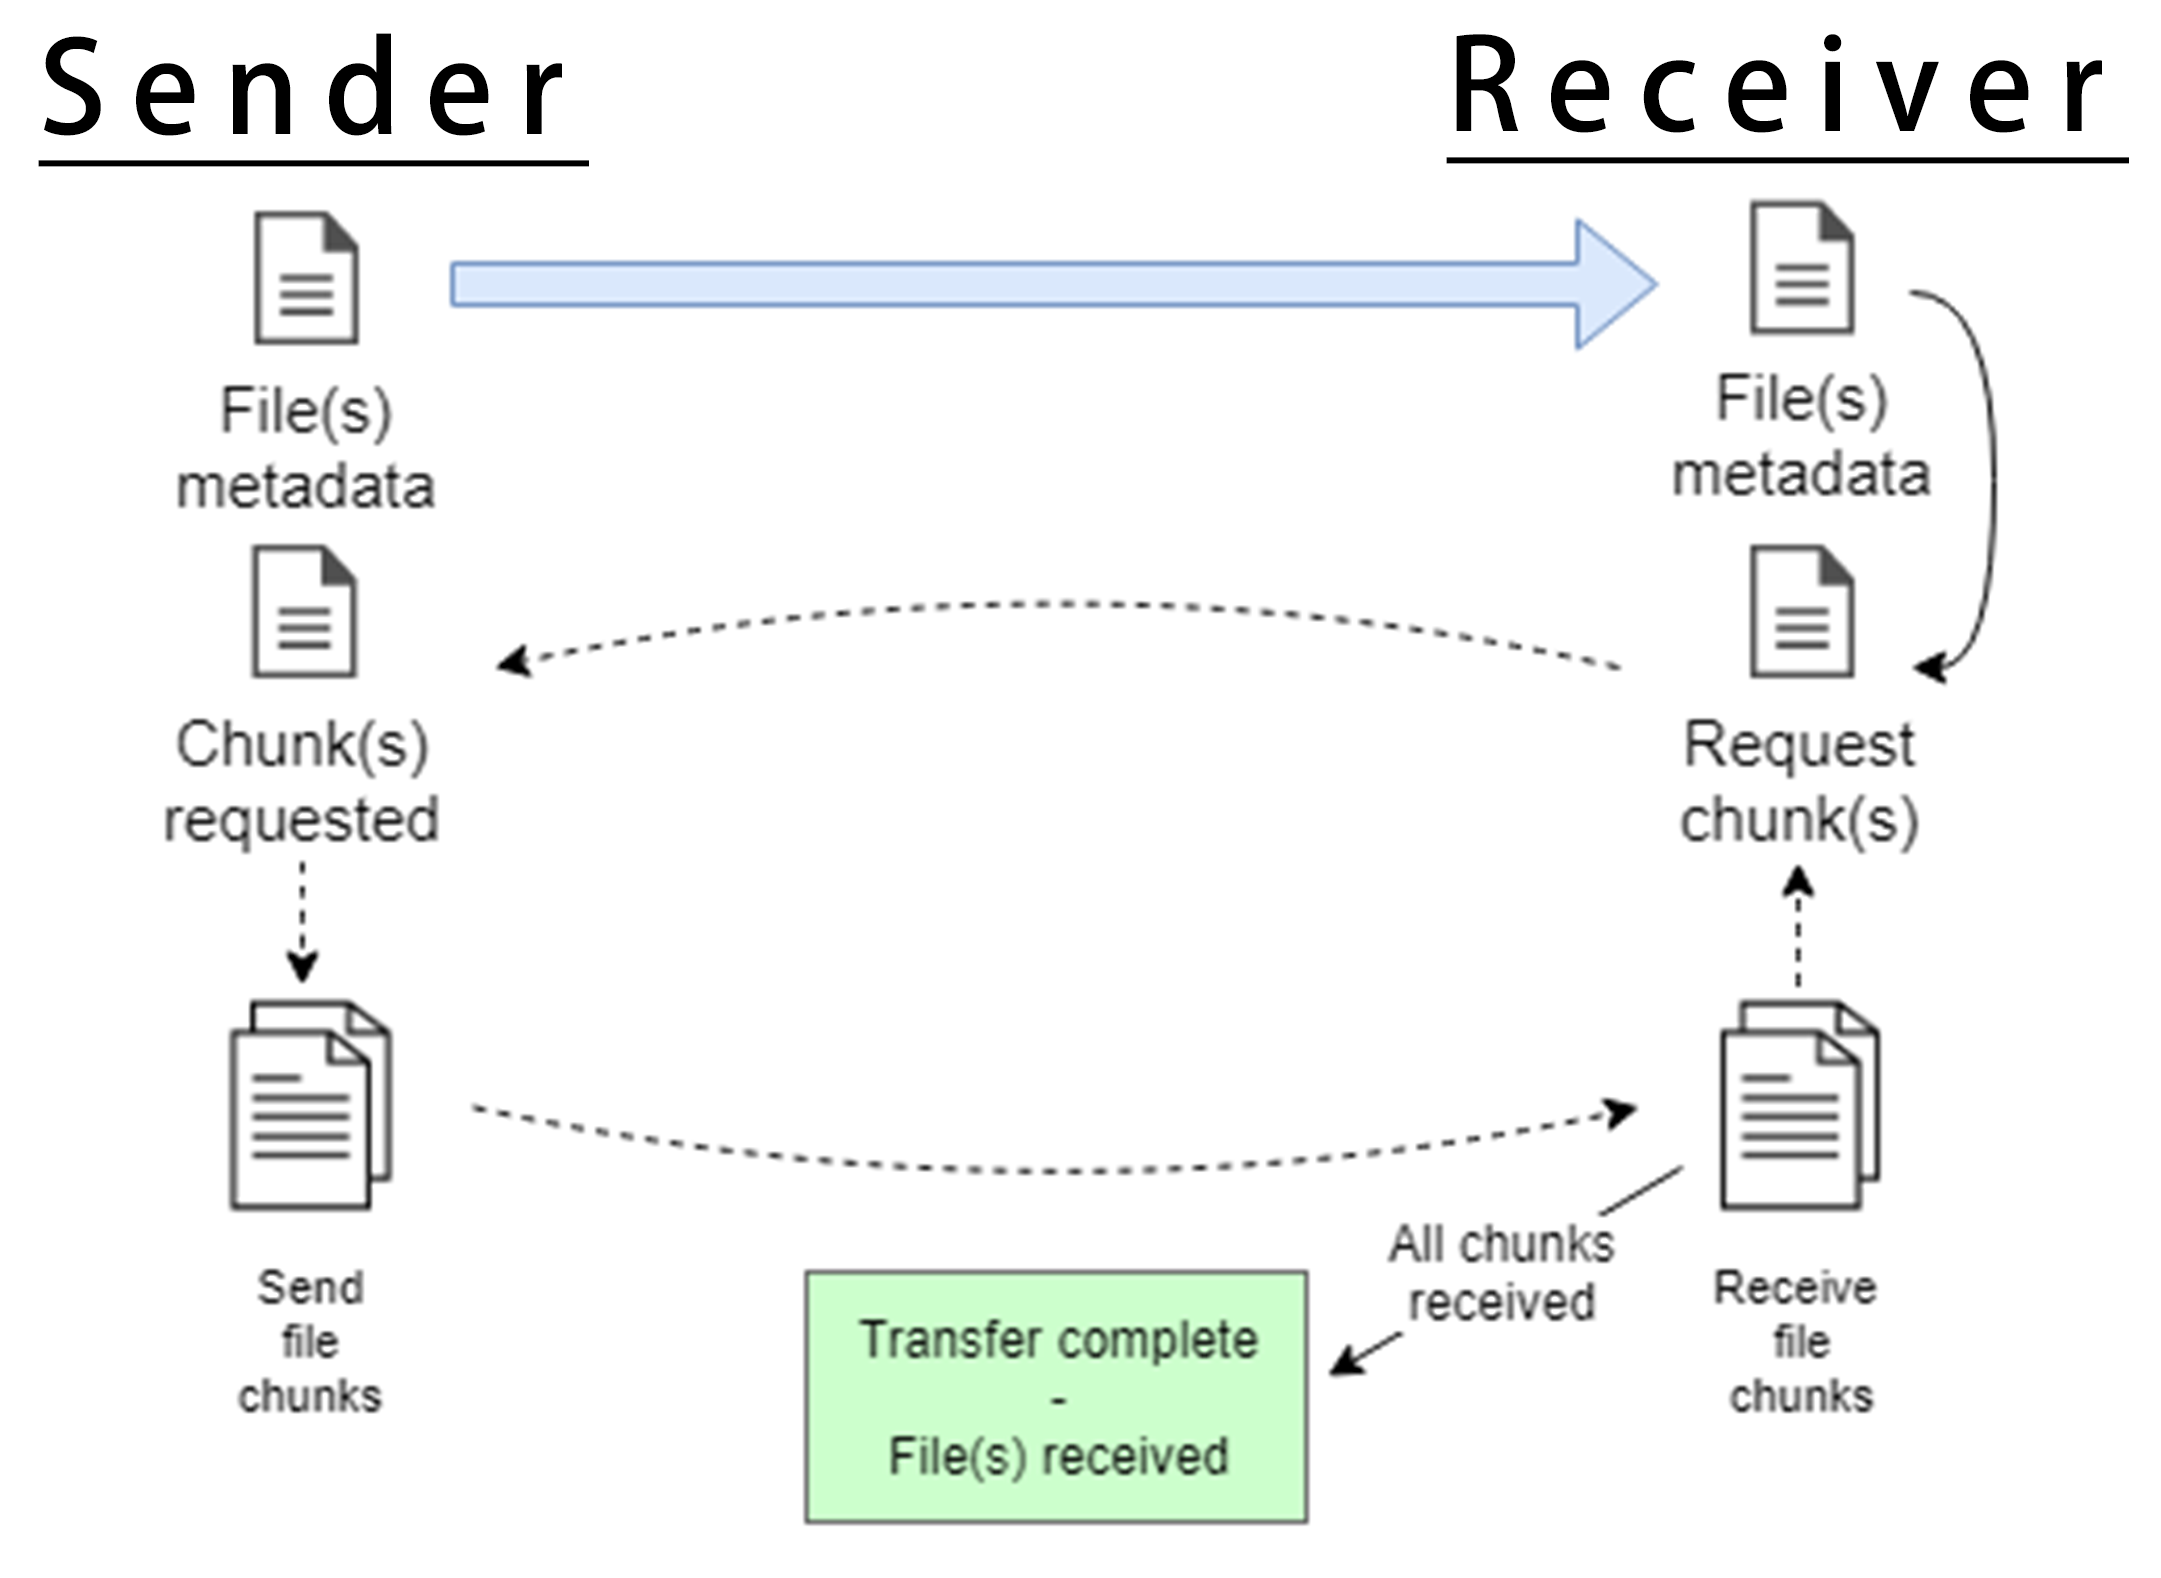
\includegraphics[width=100mm]{Figures/File_share_protocol}
		  \decoRule
		  \caption[File sharing process]{This illustrates the process of transferring file(s).}
		  \label{fig:file_off}
		\end{figure}

		The file is always transferred over a secure P2P-channel and with end-to-end encryption. It is transferred using the protocol mentioned in the section above, to manage the transfer.

		%Chunking & Size limit
		The communication will consist mostly of file-data, and as such it is interesting to know how much data can be handled. In theory, splitting files in to chunks during reading and then transferring these chunks allows for infinitely big transfers. The default max size for NodeJS is approximately 1 GB for 32-bit machines and 2 GB for 64-bit machines. This indicates the maximum amount of data that can be kept in memory. The reason for this limit is because this is the max amount of data the V8 Javascript engine used by NodeJS can have in memory at the time \cite{url_node,url_v8}.

		The current functionality separates each file in to chunks of 1200 bytes, as is the limit implemented by the Chromium implementation of WebRTC \cite{SctptransportCcCode}. The max file size is set to 160 megabytes during development, since it was the max size recommended by PubShare. It is likely that this can be increased without any issues, since NodeJS has support for keeping larger files in memory, but it would require some testing before being ready to deploy. See \Cref{fig:file_off} for an illustration of the explanation done above.

		Implementing support for bigger files, which means additional chunking, should be trivial. As a result, transport of data larger than the current limitations was not implemented. If this becomes necessary in the future, it can be added as an extra feature.
		
		%File manager
		The chunking, as well as managing which files are to be sent and which files have been received is done by the File Manager. The File Manager reads a file in to memory, then separates the data in to chunks. These chunks are then sent to through the P2P channel. Once the recipient has received all the chunks, indicated by the metadata previously received, the transfer of that file is regarded as complete. This triggers the chunks to be combined into the original file, and then stored on the recipients computer. It also notifies the sender to start transfer of the next file, or that the transfer is complete.

	\subsection{Modes}
	%TODO review
		SendIt operates with two unique modes. One is the ACS mode, which acts as a helper in establishing the P2P connection. On the other hand you have the serverless mode, which leaves everything to the end user. What is important to note is that these modes can be switched between as the user sees fit. It will also retain information used and gathered in one mode, and utilize it for future connections in the other mode as well. What it cannot do, is transfer data from one endpoint in one mode, to another endpoint in a different mode. Both endpoints have to be in the same mode, to be able to establish a connection. They can however, switch modes and still connect at a later time, as long as they both utilize the same mode. These modes will be further discussed in \Cref{Chapter4}.

	\subsection{Application}
		SendIt is developed in Javascript utilizing the Electron framework. These technologies were chosen because they allow for easy implementation while supporting multiple operating system.  It also allows for easy connection setup and direct communication via P2P. In addition it also allows for the use of existing libraries and standardizations developed for web-browsers, camouflaged in the appearance of a normal application. 

		By this we mean that the user does not need to open their web-browser to utilize SendIt, but can install it and run it like they would run any desktop program with a GUI. It also allows for easy creation of an installer file, which means the end user only needs to download and run the installer, for the program to be usable.

		%
		\begin{figure}
		\centering
		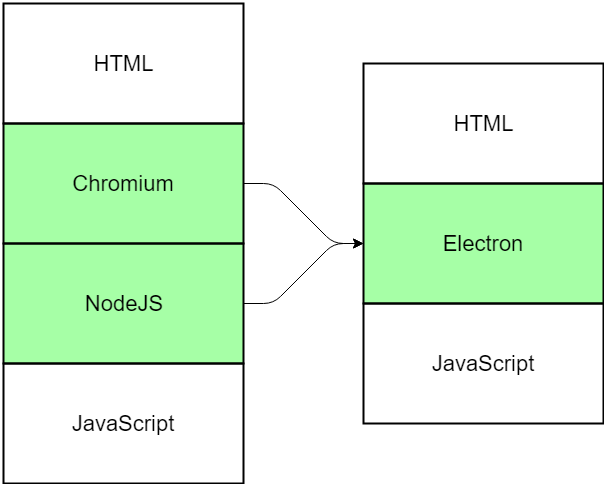
\includegraphics[width=60mm]{Dev_Stack_New}
		\caption[Application stack]{The stack for the prototype application. It is built using HTML, Electron and Javascript.}
		\label{fig:dev_stack}
		\end{figure}

		The electron framework uses NodeJS for the back end and Chromium for the front end \cite{url_electron}. In practice, this means that we are using: HTML, Electron and Javascript, where Electron uses Chromium and NodeJS. (see \Cref{fig:dev_stack}) This allows us to use modules and frameworks from any of the entities mentioned above, independently. Our implementation uses these libraries and frameworks:
		%
		\begin{itemize}
		\item NodeJS API - Used for reading and writing to disk, and finding correct files and folders \cite{url_node}
		\item Chrome Web Cryptography API - Handling the creation and exportation of keys, encryption and decryption \cite{ar_webcrypto,url_webcr_supp}
		\item NodeJS Clipboardy - Used to automatically copy the generated offer/answer to the clipboard \cite{url_clipboardy}
		\item NodeJS Electron-prompt - Used to create pop-ups for requesting input \cite{url_ele-prompt}
		\item Chrome Native WebRTC - Used for creating and managing WebRTC connections \cite{url_webrtc_chrome}
		\item jQuery v3.2.1 - Managing front-end actions and dynamic updates \cite{url_jQuery}
		\item Bootstrap v3.3.7 - Managing front-end modules and dynamic updates \cite{url_bootstrap}
		\end{itemize}
		%

%
\section{Program flow}
\label{sec:progflow}
%Program Flow
%TODO review
The general appearance of the program will be explained in the following section. The parts which are unique for each mode, will be discussed in \Cref{Chapter4}. That means that the actual functionality is not explained here, but rather the installation, setup and settings available.
%
	\subsection{Installation and launching application}
	%Installation and launch
		%Screenshots and explanation
	The application comes in the form of installer files for Linux, Mac and Windows. These files are in the format of \emph{.deb} for Linux, \emph{.dmg} for Mac and finally \emph{.exe} for Windows. The installers are very basic and requires no interaction except executing them. After that is done, the image shown in \Cref{fig:inst} will appear and run a small animation. Afterwards, SendIt is installed and will be available. In most cases, the icon will be available on the desktop. Once the application is launched for the first time, a popup window will appear, like indicated in \Cref{fig:popup}. Afterwards, the user is taken to the Home screen. This popup window will only be displayed the first time the program is opened.
	\begin{figure}[H]
		\centering
		
\includegraphics[width=\textwidth]{Figures/Base/installer}
		\decoRule
		\caption[Install animation]{While the installation of SendIt is ongoing, this small box with basic animations will appear. Once it disappears, the program is installed.}
		\label{fig:inst}
	\end{figure}

	\begin{figure}[H]
		\centering
		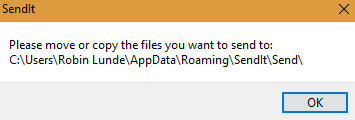
\includegraphics[width=\textwidth]{Figures/Base/start_up}
		\decoRule
		\caption[First time popup]{This popup appears the first time the program is started. It informs the user of the default location of the upload folder. This is where the files the user wants to send, should be places.}
		\label{fig:popup}
	\end{figure}	
	%
	\subsection{Home screen}
	%Home screen
		%Screenshot & explanation. Include popup!
	The home screen is the first screen the user sees. On this screen, there is not much detail or information. The logo and acronym for SendIt is displayed, as well as the navigation bar. From here on, it is all about choosing the desired functionality or tweaking the settings to fit the users desire. The only difference between the home screen for the two modes, is the formatting of the word 'Serverless' at the bottom of the screen, as well as the ACS mode not having a receive button on the navigation bar.
		\begin{figure}[H]
		  \centering
		  
\includegraphics[width=\textwidth]{Figures/Base/Home_Screen}
		  \decoRule
		  \caption[Home screen ACS mode]{The home screen displayed when the application is in ACS mode. The navigation bar has no button for receiving files. The 'serverless'-part of SendIt's acronym is also crossed out, at the bottom of the page.}
		  \label{fig:hs_acs}
		\end{figure}

		\begin{figure}[H]
		  \centering
		  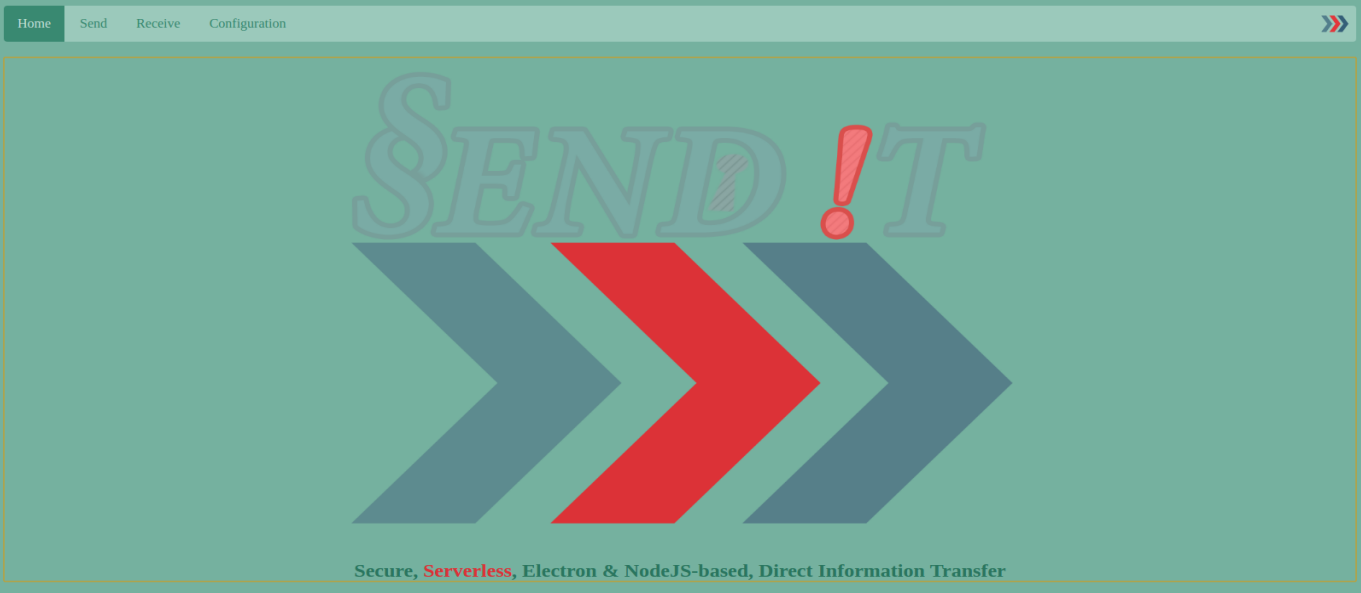
\includegraphics[width=\textwidth]{Figures/Base/Home_Screen_SL}
		  \decoRule
		  \caption[Home screen Serverless mode]{The home screen displayed when the application is in serverless mode. The navigation bar has a button for both sending and receiving files.}
		  \label{fig:hs_sl}
		\end{figure}

	\begin{figure}[H]
		  \centering
		  
\includegraphics[width=\textwidth]{Figures/Base/navbar_sl}
		  \decoRule
		  \caption[Navigation bar (Serverless mode)]{The navigation bar displayed in Serverless mode. The receive-button is not present in the ACS mode, since a separate page will be displayed if someone offers to send file(s) to you. This bar is always displayed at the top of the window.}
		  \label{fig:hs_nb}
		\end{figure}
	%
	\subsection{Settings}
	%Settings screen
		%Screenshot and explanation.
		The base view of the settings page is represented in \Cref{fig:sett}. At the top one can input which identity (or e-mail address if you will) to use. Further down, one can remove the configuration file, the file which stores all the data about which identity and which settings to normally use. Following are radio-buttons where one can choose which mode to use, as well as if one wants to use custom locations, for example for where downloaded files are stored. At the bottom, information about the current settings are displayed. Finally, there is a save changes button, to store the changes made.

		In \Cref{fig:set_det}, more detailed options are displayed. These appear when clicking the non-default option of the radio-buttons. If the ACS option is selected for \emph{Mode selection}, the field for indicating the address of the server is displayed, as well as a save button and a reset button. Afterwards, there is an option for manually selecting a file from which to load keys. One can also remove the file currently used, by pressing the 'remove ALL current keys!' button or remove individual keys by pressing them. Finally, one can customize the download and upload folder location.
		%Base screen
		\begin{figure}[H]
		  \centering
		  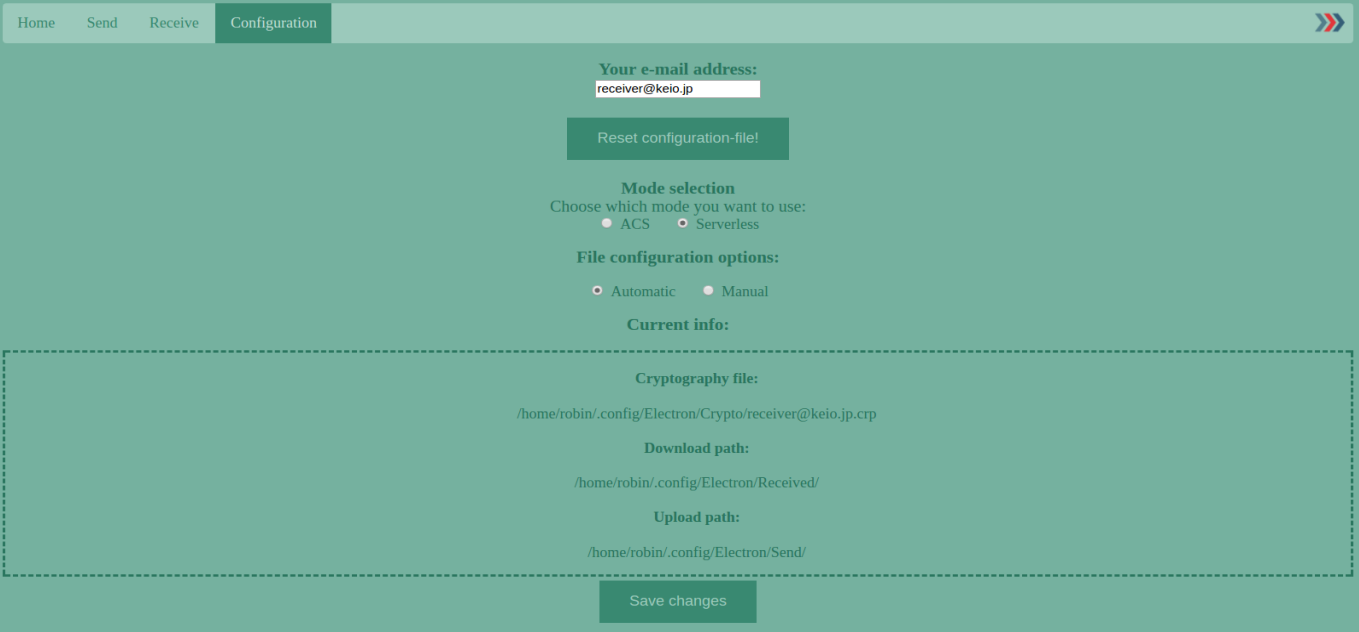
\includegraphics[width=\textwidth]{Figures/Base/Settings}
		  \decoRule
		  \caption[Settings screen]{The screen used for indicating user preferences,  upload and download location, identity management and mode selection.}
		  \label{fig:sett}
		\end{figure}

		%Details screen
		\begin{figure}[H]
		  \centering
		  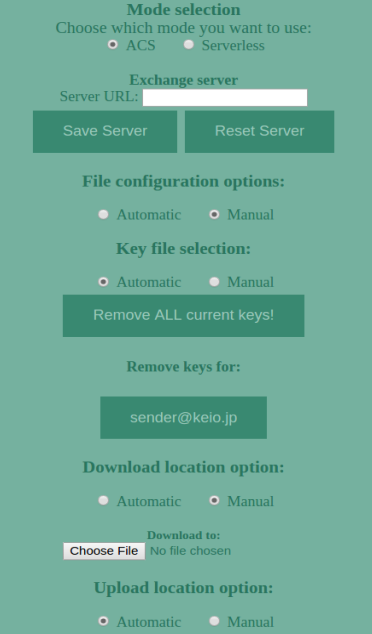
\includegraphics[width=80mm]{Figures/Base/settings_expanded}
		  \decoRule
		  \caption[Detailed settings screen]{The expanded version of the settings screen with the selection and menus displayed.}
		  \label{fig:set_det}
		\end{figure}

%
\section{ACS Server design}
\label{sec:acs_serv}
%ACS Server
%TODO review
The ACS server is in charge of forwarding information from one endpoint to another. It also has some other functionality, like authenticating identities, for the sake of forwarding information to the correct endpoint. The function of this server is kept minimal and should be easy to manage. It is also easily extendable and deployable, which makes it easy for users to host their own, for their own needs, if they for any reason do not trust any available service.
%
	\subsection{Authentication}
	\label{sec:wsprot_auth}
	%Authentication
		%How? Setup? Usage?
		The authentication scheme for the ACS server is extremely simple and just meant as an example for more sophisticated solutions. It works by having the ACS server create a symmetric key and encrypt it using the endpoints public key. To prove to the server that the endpoint could decrypt the session key, it encrypts it's own identity (e-mail) using the symmetric key and sends it back. If the identity matches the one stored, then the endpoint is authenticated. If it is the first time an endpoint connects to the server, the endpoint shares their public key and identity with the server. The server then generates a symmetric key, encrypts it with the public key supplied, and shares it with the endpoint.	%ILLUST TODO!
		
		The reason for incorporating this in the server is that forwarding data to the wrong endpoint could potentially reveal information not meant for that identity. As such, some basic form of authentication should be added to ensure that the information ends up at the right identity. This authentication does not replace or interfere with the regular authentication between endpoints in any way. It is simply a feature added to make sure the data arrives at the intended endpoint.
	%
	\subsection{WebSockets}
	\label{sec:acsws}
	%WS
		%How is it used, secure, advantage
		All communication between endpoints and the ACS server is done over WebSockets using HTTPS. This enables bi-directional communication at any time and gives an easy interface to use for communicating. The communication is exclusively done using the protocol described in the next section. No code needs to be sent from the ACS server to the endpoint in order to communicate, since all the code is pre-programmed in the client software. As such the server cannot manipulate or control the clients behavior in any way, except those intended by the protocol. The WebSocket interface and API also allows for easy handling and management of clients. Clients can connect and disconnect randomly without effecting the service as a whole. All clients are treated equally and it is easy to address each client individually. Because of this, it is very easy to receive information from one client and immediately forward it to the intended recipient. 

	%
	\subsection{ACS Protocol}
	\label{sec:wsprot}
	%
	\begin{figure}[th]
	  \centering
	  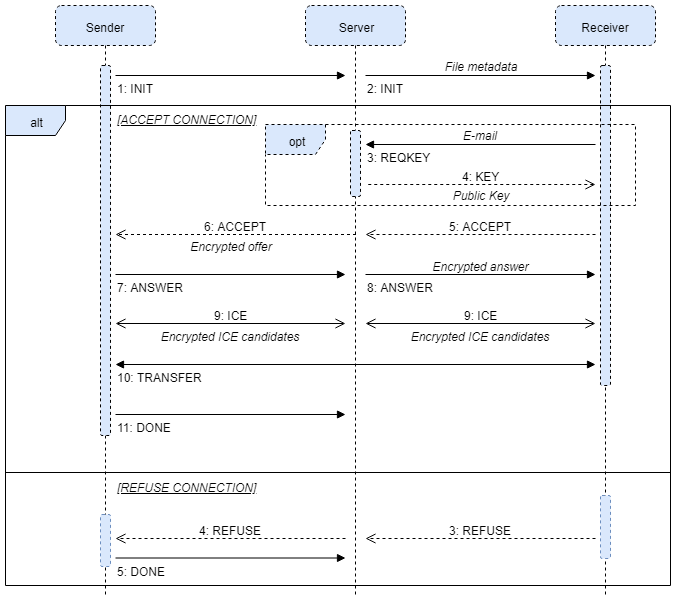
\includegraphics[width=\textwidth]{Figures/ACS_Prot/Communication}
	  \decoRule
	  \caption[WS protocol: Communication]{This is the main functionality and flow when using ACS mode to transfer files. Do note that the area marked OPT is not implemented.}
	  \label{fig:prot_comm}
	\end{figure}

	%TODO review
	The protocol used to negotiate and broker a connection in the ACS mode is made specifically for use with WebRTC. It is kept as minimal as possible, with some of the functionality left not yet implemented. This functionality is not necessary, but would improve the system by a lot. The basic format of every interaction is like shown in \Cref{tab:basic}. That means that when specifying arguments in the description of each function in the protocol, we are talking about the information going in the data-field. For an overview of the general communication flow, once authenticated and properly connected, see \Cref{fig:prot_comm}. This is where the main functionality of the ACS server is shown.
	%
	\begin{table}
		\caption{Basic protocol format}
		\label{tab:basic}
		\centering
		\begin{tabular}{l l l l}
	        \toprule
			\tabhead{Field Name} & \tabhead{Type} & \tabhead{Description} & \tabhead{Required} \\
			\midrule
			Function & String & Name of function & Yes\\
	        Origin & String & E-mail address & Yes\\
	        Destination & String & E-mail address & No\\
	        Data & JS Object & Relevant data & No\\
			\bottomrule\\
		\end{tabular}
	\end{table}
	%
	\paragraph{}
	%
	\begin{figure}[th]
	  \centering
	  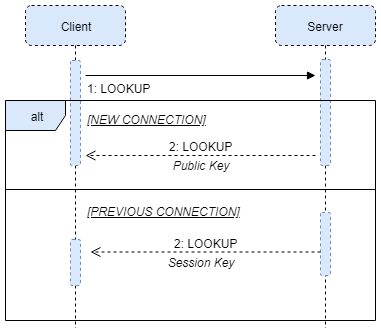
\includegraphics[width=80mm]{Figures/ACS_Prot/Connect}
	  \decoRule
	  \caption[WS protocol: Lookup function]{The lookup function exists so that the endpoint knows whether to start an authentication setup or an authentication process with the server.}
	  \label{fig:prot_lookup}
	\end{figure}

	\subsubsection*{Lookup}
	The first interaction between the client and the server is the lookup message. The client connects to the server over a WebSocket connection and sends a lookup message. This message contains the identity's e-mail address. If the server has previously communicated with the identity, it will create and send a session key (symmetric key) encrypted using the key associated with the identity. If it has not previously communicated with the identity, the servers public key is sent.% The format of these messages is shown in \Cref{tab:lookup}.
	The flow of this procedure is shown in \Cref{fig:prot_lookup}. This functionality is necessary so the endpoint knows if it should initiate an authentication setup (if there is no associated key in the server) or an authentication process (if there is an associated key in the server).
	%\begin{table}
	%	\caption{WebSocket lookup}
	%	\label{tab:lookup}
	%	\centering
	%	\begin{tabular}{l l l l}
     %   \toprule
	%	\tabhead{Name} & \tabhead{Type} & \tabhead{Argument details} & \tabhead{Required} \\
	%	\midrule
	%	Res & Boolean & True if a key is associated with the received identity & Yes\\
	%	A & as & asss & \\
	%	A & as & asss & \\
	%	\bottomrule\\
	%	\end{tabular}
	%\end{table}

	%
	\begin{figure}[th]
	  \centering
	  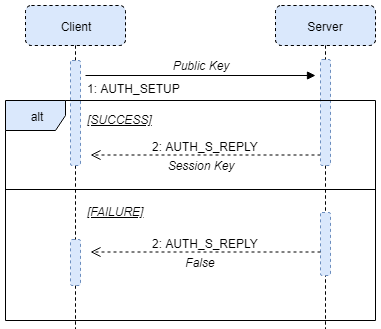
\includegraphics[width=80mm]{Figures/ACS_Prot/Auth_Setup}
	  \decoRule
	  \caption[WS protocol: Authentication setup]{This shows how the authentication setup happens and the data which is exchanged between the server and client in the two scenarios. The setup fails if the ACS server already has information stored for the given key or e-mail address.}
	  \label{fig:prot_setup}
	\end{figure}	

	\subsubsection*{Authentication Setup}
	The authentication setup between a client and the ACS server is illustrated in \Cref{fig:prot_setup}. This happens the first time an identity communicates with an ACS server and allows the ACS server to be sure that it is always communicating with the same endpoint for that identity. The endpoint sends its public key attached to a Authentication setup message, to the server. The server then checks if the e-mail is already registered. If it is, it notifies the endpoint by sending a Authentication setup reply that indicates the result as False. This means the setup failed. If the setup is successful, the server returns a symmetric key. This symmetric key is encrypted with the endpoint identity's public key, as part of the authentication. % The possible arguments used by the Authentication setup and Authentication Setup Reply messages are shown in respectively \Cref{tab:prot_auth_set} and \Cref{tab:prot_auth_set_rep}

	%
	\begin{figure}[th]
	  \centering
	  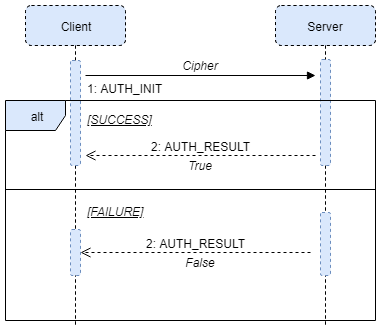
\includegraphics[width=80mm]{Figures/ACS_Prot/Auth_Init}
	  \decoRule
	  \caption[WS protocol: Authentication]{This shows how the server authenticates the user. If the decrypted cipher matches the expected value, the authentication is successful.}
	  \label{fig:prot_auth}
	\end{figure}

	\subsubsection*{Authentication}
	The authentication is done as described in \Cref{sec:wsprot_auth}. The endpoint encrypts it's e-mail address using the symmetric key, and sends it to the server. The server then decrypts the cipher and compares the e-mail stored to the one received. If there is a match, the authentication is successful, and an Authentication reply message is sent indicating the result as True. If it does not match, False is returned, and the connection dropped. See \Cref{fig:prot_auth} for a diagram of the above process. %\Cref{tab:prot_auth} and \Cref{tab:prot_auth_rep} shows the possible arguments for this functionality. 
	
	\subsubsection*{Init}
	Once the endpoint has been authenticated by the server, it is available to receive offers and send offers. This is where the Init functionality comes in. This is an offer to send files to an identity. It contains information about who the sender is, who the intended recipient is, and metadata about the file to be shared. See \Cref{fig:ACS_rec} for an example. If the server receives this type of request, it is forwarded to the indicated endpoint. The file metadata can be end to end encrypted without impacting the functionality.

	\subsubsection*{Accept}
	Once an endpoint receives an offer to receive files (in the form of an Init packet), the user has the choice to accept or refuse the connection. If the user accepts, an accept-packet containing a WebRTC offer is sent back, through the ACS server.

	\subsubsection*{Refuse}
	In the same way as explained for the Accept functionality, the Refuse functionality declines the offer to connect to the other endpoint. It terminates the connection setup between the two identities.

	\subsubsection*{Answer}
	If the Sender receives an Accept packet, it means the other endpoint accepted the connection. As such, the Sender processes the WebRTC offer received, and generates a WebRTC answer. This is then shared back to the Recipient, through the ACS server.

	\subsubsection*{ICE}
	Since this solution utilizes ICE-trickling (Described in \Cref{sec:webrtc_icetri}), it needs a protocol to continuously share ICE candidates between the two endpoints. This function exists to allow the sharing of such candidates. In other words, the ICE candidate is attached as the data portion of the ICE packet.

	\subsubsection*{Done}
	This functionality indicates that the previous connection, for whatever reason, has ended. If one endpoint sends such a packet to the ACS server, the server should consider both endpoints available for new connections.

	\subsubsection*{Error}
	If for any reason an error occurs on either side, this functionality allows for sharing what went wrong with the other endpoint. As such, the reason for the error is added to the data portion of the packet. There is no requirement to share error messages with the connection partner, but it can be useful to be able to discern between an intended pause/stop in the connection, or if something went wrong.

	\subsubsection*{Wait}
	This functionality is primarily aimed at allowing semi-asynchronous communication. It is used as a message to the endpoint from the ACS server, if they try to reach an identity currently connected to another endpoint. This indicates that the intended recipient is busy, but online, so try again later. Or if one implements queuing, wait until the endpoint is ready and automatically connect then.

	%Bla bla bla not 100% needed. Include?
	%\subsubsection*{ReqKey}
	

	%\subsubsection*{Key}


		% NOT INCLUDED IN GRAPHIC
		%
		%	ERROR & Error & asss & When an error occurs, this option is used to inform the ACS server and the other endpoint\\
		%	WAIT & as & asss & asssss\\
	
	%Protocol description:
		%name of command
		%arguments
		%Explained arguments
		%Explained functionality

		%Init
		%
		%
		%Starts the connection with that endpoint

	%Forwarding
	%TODO Review
	\subsection{Forwarding}
	The ACS is a service the exclusively does forwarding of information, whether encrypted or not. This is done by having the sender, recipient and type of communication unencrypted. The server needs this information to be able to handle the requests, and as such these fields are left in cleartext. Using this information, the ACS picks the correct functionality and executes it. For most functionality, that is just forwarding the information to the correct endpoint. It does however, need to authenticate the user, and take care of that authentication setup as well, so it does have some more functionality than just forwarding information.
	
	%
	%Semi-asynchronous transfer
	%TODO Review
	\subsection{Semi-asynchronous transfer}
	The ACS solution can allow for Semi-asynchronous messaging. What is meant by this is that one can issue the connection request, and let it be handled once the other endpoint comes online. It also allows for queuing system that stores requests and handles them in First-In-First-Out order. This still requires the sender to be online, connected to the ACS and available for transfer. As such, while the actual transfer is synchronous, the request and user interactions are not, thus 'Semi-asynchronous'.

	This brought forward the need for the wait and busy functionality in the protocol, as well as a queue of jobs for each connection, temporarily kept in the ACS server. This type of transfer is not implemented in SendIt, but some of the frameworks and systems needed for such functionality is implemented and ready to be used.

	%Add server application reletad information, like frameworks & implementation specifics?

%TODO Review name
\section{Extendability and improvements}
%SendIt as a platform!
%
In this section the extendability of SendIt in general, will be assessed. SendIt can be used as a platform to build other solutions, and as such it should be noted in what way this can be done, and how one stands to benefit from doing it.

	\subsection{Key-storage encryption}
	The file where keys are stored should be encrypted and password protected, or otherwise access restricted. The key file should only be usable, if the correct password is provided. If the wrong password is provided, the keys can not be accessed. This allows users to change the password used to store keys between each use and also makes it easy to update information regarding each key. In addition it gives no guarantee that the same encryption is used each time, which makes attacks over time harder to execute, since there is no reliable way to analyze changes or patterns in the way the file is stored. This is functionality that should be implemented and would improve the solution.

	\subsection{E-mail verification}
%E-mail verification
	One way to extend the current functionality is to add e-mail verification to the process of registering with an identity. This would increase the trustworthiness of each identity since proving ownership of the registered e-mail address would be a necessity. It would however, also include all the issues stemming from how the e-mail system is implemented. It would also make the registration process harder and require more from the users before being able to use the system. Because of these issues, it is not included in the system by default, but can easily be added. It is left up to the end-users to develop and extend the proposed system, if such functionality is a desired addition.

	\subsection{WebRTC IDP inclusion}
%WebRTC IDP
	WebRTC comes with a suggested standard for Identity Provider implementation. This is a way to corroborate someone's identity, from a service that is trusted. An example can be connecting their Facebook-account to the current identity in use, as a means for the other endpoint to verify the identity. This is possible for many different services and can be a means of increasing trust in identities. Currently, there are some arguments and disagreements on how this should be implemented in WebRTC, and as such there is not a lot of existing frameworks that can be used. This is expected to change, and at that point, using these services will allow for an easier way to increase trust in endpoints.

	The trust is of course reliant on the end-user already trusting the service that is used as the identity provider, and that the identity is as expected. As an example:\\
	If the Identity Provider used is a known service (Like Facebook), one can reasonably trust the data received. If it is from a service unknown to the user, then the identity provision does not increase the trust at all, since the data may be created for malicious purposes. In the same way, if the endpoint is expecting to be communicating with Alice, but Bob's identity is asserted by the provider, the end user should be sceptical.

	In summary, this functionality would allow to link accounts from other, independent services with your WebRTC connection, to corroborate the endpoints identity and increase trust.

%SendIt 
	\subsection{Support for bigger files}
		Supporting bigger files, can be achieved by reading in chunks of the file. Then once a chunk is completely transferred, the next chunk is read in to memory. This will allow both endpoints to handle smaller amounts of data at the time, whilst still having transmitted the whole file after the transfer of all chunks have been completed. It is not recommended to implement this until after the 'resume transfer'-feature is implemented, as transferring large amounts of data without any way of resuming it in case of failure, is less than optimal.

		The 'resume transfer' function can be easily implemented based on a communication record. Since every identity will have a list of previously transferred files, it will have the file name included. If the transfer is not completed, information about which chunk of the file was the last to be received, can be stored in this record and the endpoint can request the transfer to be continued from there.

		If the sender is not willing to resume the previous transfer, it can either start over, or another file can be transferred. This decision is up to the sender's settings and/or choices. If the sender choses to not resume the transfer, the data previously stored on the receivers local system should be removed, and the record updated as a failed transfer. The system should only allow for the requested file to be shared on the subsequent connection. An example to illustrate:

		Alice tries to send Bob File A, but the connection is broken. If Alice tries to send File A again, it will resume from the last chunk received. If it fails again, it will also allow for the transmission of File A to be resumed. However, if Alice contacts Bob again, but tries to send File B this time, the previously transmitted information (File A) stored by Bob should be removed.
		%
		\begin{table}
		\caption{Record of communication fields}
		\label{tab:comm_rec}
		\centering
		\begin{tabular}{|c|c|c|c|c|}
		\hline
		Field: &  Name & File(s) & Date & Completed\\
		\hline
		Example: & test@email.com & picture.jpg & 2018-03-20 & 0\\
		\hline
		\end{tabular}
		\end{table}
		%
		The record of communications can be implemented by creating a log that contains the fields indicated in \Cref{tab:comm_rec}. The last field can be either be -1 (meaning failed), 0 (meaning success) or the last received chunk. This is useful for being in compliance with the GDPR, allowing the user to keep track of their interactions, for reviewing their activity, and implementing a resume-transfer functionality, as mentioned above.

	\subsection{SendIt as a platform}
	%
	This is an interesting idea, since the proposed system allows for connection setup and identity assertion. One can use SendIt for this functionality and build any kind of additional functionality on top, if so desired. Especially combining with VOIP, which WebRTC is often used for, can be useful. It allows the developers to focus on their services and additional functionality, while allowing the easy to use and secure setup of the proposed system to take care of identity management and authentication. The system is modular and one can easily only use the parts desired, without much change necessary. This makes it easy to take advantage of the parts one wants, while discarding those not useful to the specific scenario at hand. 